\documentclass[11pt]{article}
\usepackage[margin=2.5cm]{geometry}
\usepackage{amsmath,amssymb,amsthm}
\usepackage{booktabs,graphicx,url,natbib,setspace}
\usepackage[colorlinks,citecolor=black,linkcolor=black,urlcolor=black]{hyperref}
\theoremstyle{plain}
\newtheorem{theorem}{Theorem}
\newtheorem{proposition}{Proposition}
\theoremstyle{definition}
\newtheorem{remark}{Remark}
\newcommand{\E}{\mathbb{E}}
\newcommand{\Prob}{\mathbb{P}}
\setstretch{1.08}

\title{Level roughness breaks anytime-valid monitoring of survey series:\\ failure of independence-based e-processes and a universal alternative}
\author{Author information removed for anonymous peer review}
\date{}

\begin{document}
\maketitle

\begin{abstract}
Anytime-valid inference lets users of published survey series inspect each release and stop at any time without losing error control. Existing constructions for monitoring such series assume that sampling errors are the only noise around a smooth path. We show that this assumption is fragile. If the latent level carries even a small random-walk disturbance, which nonsampling error, panel effects and genuine short-run fluctuation all produce, then independence-based e-processes declare a change with probability tending to one as the series grows, and we give the exact rate. We construct a universal e-process for a null class that contains the random-walk level with unknown variance, an unknown scale of the published standard errors, unknown regime levels and an unknown linear trend. It is valid for every member of the class, for any mixture alternative, and it monitors a portfolio of alternatives: a change of slope and a level shift, each at an unknown wave. We quantify what robustness costs, as an oracle inequality and as a minimum detectable change. Applied to the 56 waves of the Business Trends and Outlook Survey on artificial intelligence use, the roughness is highly significant, the independence-based monitor declares changes in nearly every series simulated from the fitted null, and the universal e-process finds no evidence of a change in growth.
\end{abstract}

\section{Introduction}

National statistical offices publish short-period estimates from rolling surveys, and users read each release as it arrives, asking whether the growth of an indicator has changed. Testing at every release inflates error rates \citep{armitage1969}, and the modern remedy is anytime-valid inference: e-values and test martingales whose error control holds uniformly over time \citep{howard2021,vovk2021,ramdas2023,grunwald2024}. Applications to online experiments \citep{johari2022} and change detection \citep{shin2023} assume that the observations are, conditionally on the past, drawn from a fixed parametric family with independent noise. The natural way to monitor a published survey series in this framework is to build the e-process on the levels, with sampling errors as the only noise around a smooth latent path.

That assumption is rarely checked and it is fragile. A published estimate is the sum of a latent level and sampling error, and the latent level itself moves from wave to wave for reasons that have nothing to do with a change in the underlying growth: nonresponse and panel effects that persist, processing changes, and real short-run fluctuation. A random-walk level with a small variance is the simplest description of this \citep{harvey1989}, and it is the structure that the structural time series literature for repeated surveys uses \citep{scott1974,durbin2012}. The question we ask is what this does to anytime-valid monitoring, and what can be done.

\paragraph{Contributions.} We make three contributions.
\begin{enumerate}
\item \emph{A failure theorem} (Section \ref{sec:failure}). In an equally spaced design with a random-walk level of variance $p$ per wave and sampling variance $\sigma^2$, the standardized curvature statistic on which independence-based monitors rely has variance $1 + (p/\sigma^2)\,n^2/42\,(1 + o(1))$. Its false-declaration probability therefore tends to one as the series lengthens, for every $p > 0$, however small, and for the version with unknown scale as well. In simulation the false-declaration probability is already 0.31 at 20 waves when $p$ is less than half the sampling variance, and 0.97 at 80.
\item \emph{A universal e-process} (Section \ref{sec:method}). For a null class that contains the roughness, the scale of the published standard errors, regime-specific levels and a linear trend as unknown parameters, we give an e-process that is valid for every member of the class and monitors a portfolio of alternatives: a change of slope and a level shift, each at an unknown wave. Validity needs no assumption on how the alternative is mixed, so the construction is a template. We bound its loss against an oracle that knows the nuisance parameters and derive the minimum detectable change.
\item \emph{An application} (Section \ref{sec:application}). In the 56 waves of the U.S.\ Census Bureau's Business Trends and Outlook Survey (BTOS) on business use of artificial intelligence, roughness is highly significant (likelihood-ratio statistic 79.6), a monitor that ignores it declares two or more changes in 98 percent of series simulated from the fitted null, and the universal e-process finds no evidence of a change in growth. We compute what size of change the series could have revealed.
\end{enumerate}

\section{Setting}
\label{sec:setting}

Let $y_1, \dots, y_n$ be published estimates at release times $t_1 < \dots < t_n$ (in units of the release interval), with published design-based standard errors $s_j$, and let $r_j$ label the questionnaire regime. We write $T_j = t_j - t_1$, $D = \mathrm{diag}(s_1^2, \dots, s_n^2)$ and $W_{jk} = \min(T_j, T_k)$. The null class is
\begin{equation}
y \sim \mathcal{N}\big(X c,\ \kappa^2 (D + r\,W)\big), \qquad c \in \mathbb{R}^{p_x},\ \kappa^2 > 0,\ r \in \mathcal{R}_0,
\label{eq:null}
\end{equation}
where $X$ has one column per regime (an unknown level for each) and one column $t_j$ (an unknown common slope). Equation \eqref{eq:null} is the marginal law of $y_j = L_j + e_j$ with sampling error $e_j \sim \mathcal{N}(0, \kappa^2 s_j^2)$ and a level $L_j = L_1 + b\,T_j + \sum_{i \le j} \eta_i$ with $\eta_i \sim \mathcal{N}(0, \kappa^2 r\,(T_i - T_{i-1}))$: a linear trend plus a random walk. The parameter $r \ge 0$ is the roughness, in squared points per wave relative to the scale $\kappa^2$; $p = \kappa^2 r$ is the variance of the level disturbance per wave. The set $\mathcal{R}_0$ is a finite grid that contains zero and covers roughness from far below to far above the sampling variance; it can be refined without changing any statement below. The covariance of the first $n$ waves is the leading block of the covariance of the first $n+1$, so \eqref{eq:null} defines a family of laws on the sequence.

The null says that, apart from sampling error and a level disturbance of unknown size, the series follows a straight line within each regime. A change in growth is a departure from it. We consider two families of alternatives, each at an unknown wave $k$ and with an unknown size $\delta$: a change of slope, $\E y = X c + \delta\,(t - t_k)_+$, and a level shift, $\E y = X c + \delta\,\mathbf{1}\{j \ge k\}$. A level shift of this kind is what an unannounced instrument event looks like, and it is the alternative to which an unexplained one-wave drop belongs.

\section{Independence-based monitors fail under level roughness}
\label{sec:failure}

The natural independence-based monitor, which we use as the benchmark, tests the curvature of the series with sampling error as the only noise: a mixture e-process on the quadratic coefficient after the level and the slope have been projected out \citep{robbins1970,perezortiz2024}. Let $t_j = j$, $s_j = \sigma$ constant and $m$ the residual of $(j - \bar{j})^2$ on $(1, j)$. The curvature statistic is
\[
Z_n = \frac{\sum_j m_j y_j}{\sigma \|m\|},
\]
which is $\mathcal{N}(0,1)$ under the independence null ($r = 0$), and the e-process built on it declares when $E_n^{\pm} = \frac{2}{\tau\sqrt{a_n}}\,\Phi(\pm A_n/\sqrt{a_n})\,e^{A_n^2/(2a_n)}$ reaches $2/\alpha$, with $A_n = \sigma^{-2}\sum m_j y_j$, $B_n = \sigma^{-2}\|m\|^2$ and $a_n = B_n + \tau^{-2}$.

\begin{theorem}[failure]
\label{thm:failure}
Let $y_j = a + b j + L_j + e_j$ with $e_j \sim \mathcal{N}(0, \sigma^2)$ independent and $L$ a Gaussian random walk with increment variance $p > 0$. Then
\[
\mathrm{Var}(Z_n) = 1 + \frac{p}{\sigma^2}\,\frac{n^2}{42}\,\big(1 + O(n^{-1})\big).
\]
Consequently the probability that the e-process with prior scale $\tau$ and threshold $2/\alpha$ has declared by wave $n$ tends to one as $n \to \infty$, for every $p > 0$, $\tau > 0$ and $\alpha \in (0,1)$. The same holds for the version of the e-process with unknown scale, in which $\kappa^2$ is estimated from the residual sum of squares.
\end{theorem}

Theorem \ref{thm:failure} is proved in Appendix \ref{app:proof}. The constant $1/42$ follows from two integrals, $\int_0^1 g^2 = 1/7560$ and $\int_0^1 m^2 = 1/180$ in the scaled design, and we checked it against the exact variance for $n$ up to 320. Two features matter. The failure is not a small-sample effect and it is not removed by estimating the scale, because the roughness inflates the standardized statistic in proportion to $n^2$ and the estimated variance only in proportion to $n$, so that the studentized statistic still diverges, at rate $\sqrt{n}$. And it is not a property of a large $p$: Figure \ref{fig:failure} shows that with $p = 0.01$, under half the sampling variance $\sigma^2 = 0.0225$, the false-declaration probability is 0.31 at 20 waves, 0.76 at 40, 0.97 at 80 and 1.0 at 160, for the e-process with known scale; with unknown scale it is 0.16, 0.56 and 0.90 at 20, 40 and 80.

\begin{figure}[t]
\centering
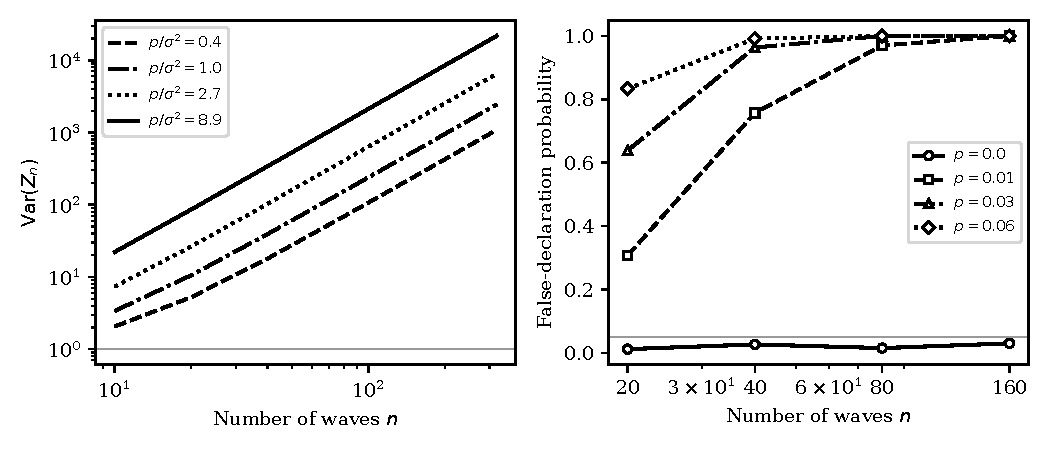
\includegraphics[width=0.62\textwidth]{fig_failure.pdf}
\caption{Probability that the independence-based e-process (known scale, threshold 40 on each of two one-sided monitors, level 0.05) has declared a curvature change by wave $n$, when the series follows a straight line with a random-walk level of variance $p$ per wave and sampling standard deviation 0.15 (sampling variance 0.0225; 600 replications for $n \le 80$, 300 for $n = 160$). The horizontal line is the nominal level.}
\label{fig:failure}
\end{figure}

\section{A universal e-process}
\label{sec:method}

\subsection{Construction}

Let $X_n$ be the design of the first $n$ waves and $R_n$ the data modulo the column space of $X_n$, that is, the residual vector $y_{1:n} - \hat{y}$ from any generalized least squares fit. Under \eqref{eq:null} the law of $R_n$ does not depend on $c$, and it has a density, with respect to a fixed reference measure on the residual space, of the restricted likelihood (REML) form
\[
P_\theta(R_n) \propto |\Sigma_\theta|^{-1/2}\,|X_n^\top \Sigma_\theta^{-1} X_n|^{-1/2}\exp\!\big(-\tfrac12\, y^\top P_\theta\, y\big), \qquad \Sigma_\theta = \kappa^2(D + rW),
\]
with $P_\theta = \Sigma_\theta^{-1} - \Sigma_\theta^{-1}X_n (X_n^\top\Sigma_\theta^{-1}X_n)^{-1}X_n^\top\Sigma_\theta^{-1}$. For a component $c = (g, f, k, \tau)$ of the alternative, with nuisance setting $g = (r_g, \kappa_g^2)$, family $f$ (slope or level), change wave $k$ and prior scale $\tau$ on $\delta$, let $z_{f,k}$ be the alternative column and
\[
Q_{c}(R_n) = P_{g}(R_n)\cdot \mathrm{BF}_c, \qquad \mathrm{BF}_c = (1 + \tau^2 b)^{-1/2}\exp\!\Big(\frac{\tau^2 a^2}{2(1 + \tau^2 b)}\Big),
\]
with $a = z_{f,k}^\top P_g\, y$ and $b = z_{f,k}^\top P_g\, z_{f,k}$. This is the density of $R_n$ under $\mathcal{N}(\delta\, M z_{f,k}, M\Sigma_g M^\top)$ with $\delta \sim \mathcal{N}(0, \tau^2)$, where $M$ projects out $X_n$. Let $Q_n = \sum_c w_c Q_c$ be a mixture with fixed weights, and define
\begin{equation}
E_n = \frac{Q_n(R_n)}{\sup_{\theta \in \Theta_0} P_\theta(R_n)}, \qquad \Theta_0 = \{(\kappa^2, r): \kappa^2 > 0,\ r \in \mathcal{R}_0\}.
\label{eq:E}
\end{equation}
The supremum over $\kappa^2$ is explicit ($\hat\kappa^2 = y^\top P_{1,r}\, y/\nu$ with $\nu = n - p_x$), and the supremum over $r$ is a search over the grid. The weights $w_c$ are uniform over two families, over the change waves $k \in \{3, \dots, n_{\max}\}$ for a planned horizon $n_{\max}$, over a grid of five roughness values from zero to 32 times the median sampling variance, four values of $\kappa_g^2$ from 0.5 to 4, and four prior scales for each family. Components whose change wave lies beyond the current wave have $z_{f,k} = 0$ on the data so far and contribute their null density.

\begin{theorem}[validity]
\label{thm:validity}
For every $\theta \in \Theta_0$, every $c \in \mathbb{R}^{p_x}$ and every choice of weights, if $y \sim \mathcal{N}(Xc, \Sigma_\theta)$ then
\[
\Prob_\theta\big(\exists\, n:\ E_n \ge 1/\alpha\big) \le \alpha.
\]
\end{theorem}

The proof (Appendix \ref{app:proof}) is short. Each $Q_c$ is a probability density on the residual space, and the family is consistent in $n$ because the covariance and the alternative columns are consistent in $n$. Hence $\Lambda_n = Q_n/P_\theta$ is a likelihood-ratio martingale for the true $\theta$ with respect to the filtration generated by $R_n$, and $E_n \le \Lambda_n$ because the supremum is at least $P_\theta$. Ville's inequality bounds $\Prob(\sup_n \Lambda_n \ge 1/\alpha)$ by $\alpha$. The argument is the one behind universal inference \citep{wasserman2020}, combined with invariance to the location nuisance \citep{perezortiz2024}; what is new is that it covers a correlated null class, which is what makes the construction robust to roughness. Nothing in it depends on how $Q_n$ is mixed.

\begin{remark}
The statement is for a finite null grid $\mathcal{R}_0$ and it extends to the continuum by replacing the grid maximum by the supremum. We use a grid of 46 values spanning four orders of magnitude, with zero added; the maximizer is not on the boundary in any of our applications.
\end{remark}

\subsection{The price of robustness}

The loss relative to a user who knew the nuisance parameters has three parts. For a component $c$ that matches the true alternative and nuisance setting,
\begin{equation}
\log E_n \ \ge\ \log w_c + \log \Lambda_{c,n} - \Delta_n, \qquad \Delta_n = \log \sup_{\theta \in \Theta_0} P_\theta(R_n) - \log P_{g}(R_n) \ \ge 0,
\label{eq:oracle}
\end{equation}
where $\Lambda_{c,n} = Q_c/P_g$ is the oracle Bayes factor: the mixture over components costs $\log(1/w_c)$, which for our weights is about $9$ nats, and the supremum costs $\Delta_n$, the gain from fitting the null nuisance parameters to the data. When the data satisfy the null at the oracle setting, $\Delta_n$ is a likelihood-ratio statistic for two parameters and is $O_P(1)$; under an alternative the null fit can absorb part of the signal, and $\Delta_n$ need not be small, which is a further source of loss. The oracle term grows linearly in the information. For a simple alternative with slope change $\delta$ at wave $k$ and known nuisance parameters, $\E\log\Lambda = \tfrac12\delta^2 b_k(\Sigma)$ with $b_k(\Sigma) = z_k^\top P\, z_k$, which gives the minimum detectable change
\begin{equation}
\delta_{\min} = \sqrt{\frac{2L}{b_k(\Sigma)}}, \qquad L = \log\frac{1}{\alpha} + \log\frac{1}{w_c} + \bar\Delta.
\label{eq:mdsc}
\end{equation}
The information $b_k(\Sigma)$ is what roughness destroys: a random-walk level absorbs everything that a straight line does not explain, and Section \ref{sec:application} shows that for the BTOS design it is 170 times smaller than without roughness.

\section{Simulation}
\label{sec:simulation}

All simulations use the dates and standard errors of the 54 legacy-wording BTOS waves, a linear mean of slope 0.12 points per wave, and level $\alpha = 0.05$ (threshold 20 for a single two-sided e-process).

\paragraph{Validity.} The probability that the universal e-process ever reaches 20 is 0.000 for independent errors, 0.000 for a standard error 1.5 times the published one, and 0.000, 0.001 and 0.000 for random-walk levels with $p = 0.03$, 0.06 and 0.2 per wave (1,000 replications each). For first-order autoregressive errors with correlation 0.3, which are outside the null class, it is also 0.000. The independence-based monitor, on the same series with $p = 0.06$, declares in every replication. The universal e-process is very conservative, as the supremum and the mixture make it; Table \ref{tab:power} shows the price.

\begin{table}[t]
\centering\small
\caption{Probability that the universal e-process declares by the last wave when the slope changes by $\delta$ points per wave, or the level shifts by $\delta$ points, at wave 25 of 54, for roughness $p$ (variance of the level disturbance per wave; the published sampling variance is about 0.02). In parentheses: the oracle that knows the nuisance parameters, the family and $\delta$ and mixes only over the change wave. 500 replications.}
\label{tab:power}
\begin{tabular}{lccc|ccc}
\toprule
& \multicolumn{3}{c|}{Slope change (points per wave)} & \multicolumn{3}{c}{Level shift (points)} \\
$p$ & 0.1 & 0.2 & 0.4 & 0.5 & 1 & 2 \\
\midrule
0 & 0.13 (0.86) & 0.97 (1.00) & 1.00 (1.00) & 0.10 (0.54) & 0.96 (0.99) & 1.00 (1.00) \\
0.03 & 0.00 (0.01) & 0.05 (0.28) & 0.82 (0.97) & 0.00 (0.00) & 0.08 (0.28) & 0.98 (1.00) \\
0.06 & 0.00 (0.00) & 0.01 (0.10) & 0.39 (0.81) & 0.00 (0.00) & 0.02 (0.08) & 0.78 (0.96) \\
\bottomrule
\end{tabular}
\end{table}

\paragraph{Power.} Table \ref{tab:power} and Figure \ref{fig:power} show how roughness removes power. Without roughness a slope change of 0.2 points per wave, nearly twice the typical growth of 0.12, is detected in 97 percent of replications. With the roughness estimated from the BTOS ($p = 0.06$) the same change is detected in 1 percent, and detection requires a change of 0.4 (39 percent) or more. A level shift of 1 point is detected at $p = 0$ and not at $p = 0.06$. The oracle shows how much of this is the price of not knowing the nuisance parameters and how much is information destroyed by the roughness itself: at $p = 0.06$ and slope 0.4, the oracle detects in 81 percent and the universal e-process in 39 percent. Equation \eqref{eq:mdsc} predicts the scale: with $b_k = 200$ (Section \ref{sec:application}) and $L = 13$ it gives $\delta_{\min} = 0.36$.

\begin{figure}[t]
\centering
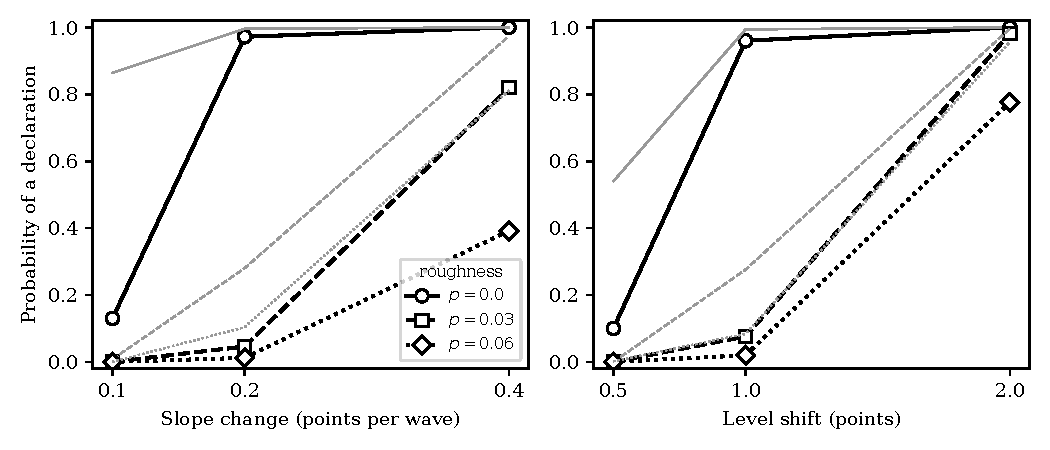
\includegraphics[width=0.95\textwidth]{fig_power.pdf}
\caption{Power of the universal e-process (black) and of the oracle (grey) for a slope change (left) and a level shift (right) at wave 25 of 54, by roughness $p$ (variance of the level disturbance per wave).}
\label{fig:power}
\end{figure}

\section{Application: business use of artificial intelligence}
\label{sec:application}

\paragraph{Data.} The BTOS is the Census Bureau's biweekly survey of about 1.2 million employer businesses \citep{censusmethod2025}. We use the 56 national waves on current use of artificial intelligence from 24 September 2023 to 14 December 2025 \citep{bonney2024}: 54 with the legacy wording and two with the wording introduced on 17 November 2025, which has its own level in the design. The estimate rises from 3.7 to 10.0 percent under the legacy wording; the published standard errors have median 0.15.

\paragraph{Roughness.} Maximizing the restricted likelihood over \eqref{eq:null} gives a roughness of $\hat{p} = 0.058$ points$^2$ per wave (profile 95 percent interval 0.018 to 0.46) and a scale $\hat\kappa^2 = 1.28$ on the published variances. The level disturbance has standard deviation 0.24 points per wave against a sampling standard deviation of 0.15. Setting $r = 0$ lowers the restricted log-likelihood by 39.8, a likelihood-ratio statistic of 79.6, so the evidence for roughness is overwhelming. Figure \ref{fig:btos} shows the fitted level, which follows the series closely.

\begin{figure}[t]
\centering
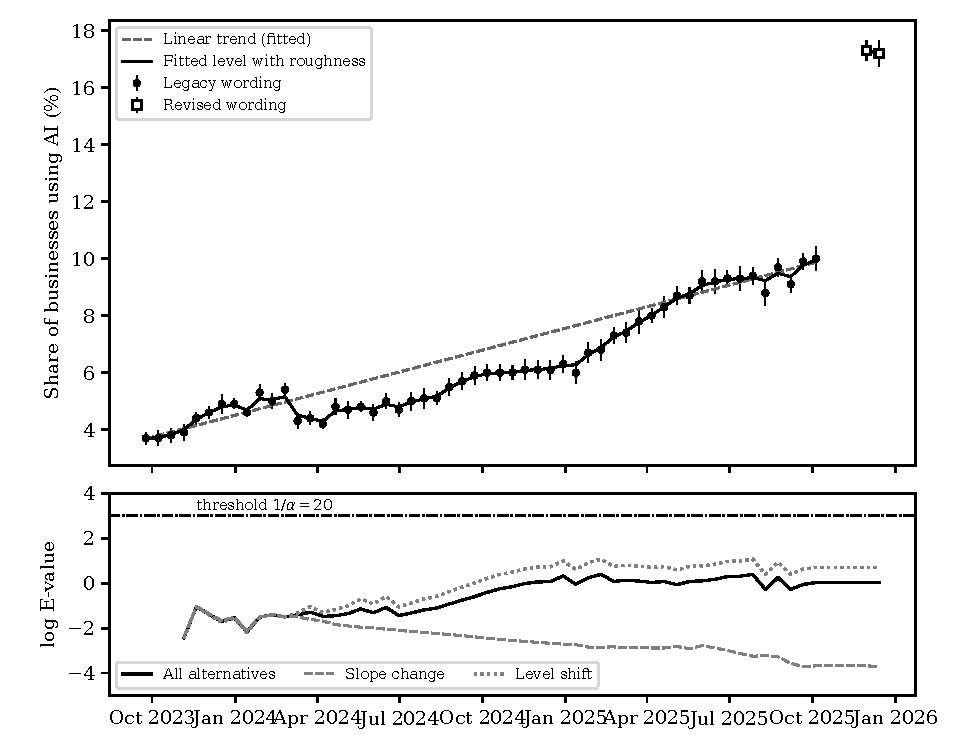
\includegraphics[width=0.78\textwidth]{fig_btos.pdf}
\caption{Top: national share of businesses using artificial intelligence with 95 percent intervals, the fitted linear trend and the fitted trend plus rough level. Bottom: log E-value of the universal e-process, for all alternatives and by family, against the threshold $\log 20$.}
\label{fig:btos}
\end{figure}

\paragraph{What an independence-based monitor would say.} The e-process of Section \ref{sec:failure}, with restarts after each declaration, declares twice on the BTOS series, on 10 March 2024 (deceleration) and 6 April 2025 (acceleration). We simulated 400 series from the fitted null: a straight line with the estimated roughness and scale and the BTOS standard errors and dates. The monitor declares at least once in 100 percent and at least twice in 98 percent of them, and 3.1 times on average. The two declarations are therefore what the fitted null produces; they are not evidence of a change in growth.

\paragraph{The universal e-process.} Applied to the same 56 waves, the universal e-process peaks at $\log E = 0.39$ ($E = 1.5$), on 9 February 2025, against a threshold of $\log 20 = 3.0$. By family, the slope alternative peaks at $-1.0$ and the level alternative at $1.07$ ($E = 2.9$); the latter belongs to the one-wave fall of 10 March 2024, which is the largest change in the series (6.2 combined standard errors) but is not enough, once roughness is allowed, to establish an instrument event. The result is not sensitive to the prior: with wider prior scales, with the nuisance mixture restricted to rough settings, with the scale fixed, with a single family, or with the legacy waves only, the maximum log E-value is between $-1.0$ and $1.3$ (Table \ref{tab:app}). In the seven employment-size classes the roughness estimates range from 0.06 to 0.94 and no class exceeds $\log E = -0.6$; the average of the seven e-processes, which is valid under any dependence between them, peaks at $-0.95$.

\begin{table}[t]
\centering\small
\caption{Maximum log E-value of the universal e-process on the BTOS national series under variants of the prior (threshold $\log 20 = 3.00$).}
\label{tab:app}
\begin{tabular}{lc}
\toprule
Variant & Maximum log E \\
\midrule
Default & 0.39 \\
Wider prior scales on $\delta$ & 0.10 \\
Nuisance mixture restricted to rough settings ($r \ge 2\times$ sampling variance) & 1.17 \\
Scale fixed at the published value & 1.25 \\
Slope alternatives only & $-1.03$ \\
Level alternatives only & 1.07 \\
Legacy-wording waves only & 0.43 \\
\bottomrule
\end{tabular}
\end{table}

\paragraph{What the series could have revealed.} For the BTOS design with the fitted roughness, the information on a slope change after wave 20 is $b = 205$ and on a level shift $b = 10$, against $35{,}000$ and $190$ without roughness. Equation \eqref{eq:mdsc} with $L = 13$ gives a minimum detectable slope change of 0.36 points per wave, three times the average growth of 0.12, and a minimum detectable level shift of 1.6 points; without roughness they would be 0.027 and 0.37. The largest change in the series by any of these measures, the March 2024 drop of 1.1 points, is below the minimum detectable level shift.

\section{Discussion}

\paragraph{What the paper shows.} Anytime-valid monitoring of a survey series is only as good as the null. If the latent level is rough, independence-based e-processes are not conservative or slightly anticonservative; they are wrong, by a margin that grows without bound, and the failure begins at roughness well below the sampling variance. A null class that includes the roughness restores validity, at a price that we measure: the BTOS series could reveal a change of growth of three times its average, not of the order of change that users ask about.

\paragraph{Limitations.} The null class is Gaussian and has one source of dependence, a random-walk level; autoregressive disturbances are outside it, and while the monitor was valid in the simulation we have no guarantee for them. The universal construction is conservative: realized false-declaration probabilities are below 0.001, so a calibrated rule would have more power, and the oracle inequality \eqref{eq:oracle} bounds the loss but not tightly. The alternative mixture is fixed in advance and uses a planned horizon. The standard errors enter as weights and are treated as fixed. We analyzed one series; the finding that the roughness is large may be specific to it, and the size classes give estimates from 0.06 to 0.94. The formal results concern the roughness and not the sampling design, and the approach does not model panel rotation. A tolerance for small departures from linearity, which would let the monitor detect change smaller than the roughness, and an extension to unknown regime dates, are open.

\paragraph{Implications.} For users, the practical rule is that a declaration from a monitor that assumes independent noise should be checked by estimating the roughness and simulating the monitor under the fitted null, as we did. For agencies, the information $b_k$ in \eqref{eq:mdsc} is a design quantity: it says how large a change a series of a given length, precision and roughness can reveal, and it can be reported with the series.

\section*{Declaration of Generative AI Use}
Generative AI tools were used to support the writing of code and to polish the language of the manuscript. The research idea, the methods and algorithms, and the interpretation of the results are the author's own. The author reviewed and edited all AI-assisted output and takes full responsibility for the content of the work.

\section*{Data and code availability}
All data are public statistics of the U.S.\ Census Bureau (Business Trends and Outlook Survey). The code reproduces every number, table and figure.

\bibliographystyle{chicago}
\bibliography{refs}

\appendix
\section{Proofs}
\label{app:proof}

\paragraph{Proof of Theorem \ref{thm:validity}.} Fix $\theta \in \Theta_0$ and $c$. Let $\mathcal{G}_n$ be the $\sigma$-field generated by $R_n$, that is, by $y_{1:n}$ modulo the column space of $X_n$; since the columns of $X_{n+1}$ restricted to the first $n$ rows span that of $X_n$ (a column for a new regime is zero on earlier rows), $R_n$ is a function of $R_{n+1}$ and $(\mathcal{G}_n)$ is a filtration. Under $\mathcal{N}(Xc, \Sigma_\theta)$ the law of $R_n$ is $\mathcal{N}(0, M_n\Sigma_\theta M_n^\top)$ on the residual space, with density $P_\theta(R_n)$ with respect to the common reference measure. Each $Q_c$ is a Gaussian (a Gaussian mixture over $\delta$) density with positive definite covariance, so $Q_n = \sum_c w_c Q_c \ll P_\theta$ on $\mathcal{G}_n$, with $\Lambda_n = Q_n(R_n)/P_\theta(R_n)$. The laws are consistent in $n$: $\Sigma_\theta(n)$ is the leading block of $\Sigma_\theta(n+1)$ since $D$ is diagonal and $W_{jk} = \min(T_j, T_k)$ does not depend on later waves, and the alternative columns restricted to the first $n$ rows are the alternative columns of $n$ waves. Hence $Q_{n+1}$ restricted to $\mathcal{G}_n$ is $Q_n$, and the same for $P_\theta$, so $\Lambda_n$ is the Radon--Nikodym derivative of $Q$ with respect to $P_\theta$ on $\mathcal{G}_n$ and a nonnegative $P_\theta$-martingale with $\Lambda_0 = 1$. Because $\theta \in \Theta_0$, $\sup_{\theta'} P_{\theta'}(R_n) \ge P_\theta(R_n)$, so $0 \le E_n \le \Lambda_n$ for all $n$. By Ville's inequality $\Prob_\theta(\sup_n \Lambda_n \ge 1/\alpha) \le \alpha$, and the event $\{\exists n: E_n \ge 1/\alpha\}$ is contained in it. $\square$

\paragraph{Proof of Theorem \ref{thm:failure}.} Let $m_j$ be the residual of $(j-\bar{j})^2$ on $(1, j)$, so that $\sum_j m_j = 0$, $\sum_j j\,m_j = 0$ and $\|m\|^2 = n^5/180\,(1 + O(n^{-1}))$. Write $S_i = \sum_{j \ge i} m_j$. Because the linear trend is in the span of $(1, j)$ it does not enter $\sum_j m_j y_j = \sum_j m_j (L_j + e_j)$. The random walk is $L_j = L_1 + \sum_{i=2}^{j}\eta_i$, so $\sum_j m_j L_j = \sum_{i=2}^n S_i\,\eta_i$ and, by independence, $\mathrm{Var}(\sum_j m_j y_j) = p \sum_{i=2}^n S_i^2 + \sigma^2\|m\|^2$. In the scaled design $x = i/n$, $S_i = n^3 g(x)(1 + O(n^{-1}))$ with $g(x) = \int_x^1 \big((u - \tfrac12)^2 - \tfrac1{12}\big)du$, and a Riemann sum gives $\sum_i S_i^2 = n^7\int_0^1 g^2\,(1 + O(n^{-1})) = n^7/7560\,(1 + O(n^{-1}))$. Therefore
\[
\mathrm{Var}(Z_n) = 1 + \frac{p}{\sigma^2}\frac{\sum_i S_i^2}{\|m\|^2} = 1 + \frac{p}{\sigma^2}\,\frac{180}{7560}\,n^2\,(1 + O(n^{-1})) = 1 + \frac{p}{\sigma^2}\frac{n^2}{42}\,(1 + O(n^{-1})).
\]
$Z_n$ is Gaussian with mean zero, so $\Prob(|Z_n| > z) \to 1$ for every fixed $z$ as $n \to \infty$, since the variance diverges.

For the e-process with known scale, $E_n^{\pm}$ takes the larger of two values and at the sign of $A_n$, $\Phi(|A_n|/\sqrt{a_n}) \ge \tfrac12$, so $\max E_n^{\pm} \ge (\tau\sqrt{a_n})^{-1} e^{A_n^2/(2a_n)}$. With $A_n^2/a_n = Z_n^2\,B_n/a_n$ and $B_n/a_n \to 1$ this exceeds $2/\alpha$ as soon as $Z_n^2 \ge 4\log\big((2/\alpha)\,\tau\sqrt{2B_n}\big) = 10\log n + O(1)$, which has probability tending to one since $Z_n^2$ is of order $n^2$.

For the version with unknown scale (a proof sketch), let $\mathrm{RSS}^{(0)}_n$ be the residual sum of squares after regressing $y$ on $(1, j)$ and $\rho_n = (\sum_j m_j y_j)^2/(\|m\|^2\,\mathrm{RSS}^{(0)}_n)$ the fraction of it explained by the quadratic direction $m$. The profile likelihood ratio of the quadratic model against the linear one is $(1-\rho_n)^{-\nu/2}$ with $\nu = n-2$, and a Laplace approximation of the mixture over the curvature gives $\log E^{\sigma}_n = \tfrac{\nu}{2}\log\{1/(1-\rho_n)\} + O_P(\log n)$. By Donsker's theorem, $n^{-1/2}p^{-1/2}L_{\lfloor nx\rfloor}$ converges to a Brownian motion $\mathbb{B}$ and $\rho_n$ converges in distribution to the squared cosine between the detrended path of $\mathbb{B}$ and the quadratic function, which is positive almost surely. For every $\varepsilon > 0$ the probability that $\rho_n > \varepsilon$ converges to $\Prob(\rho_\infty > \varepsilon)$, which tends to one as $\varepsilon \to 0$, and on that event $\log E^{\sigma}_n$ is of order $n$. Hence the probability of having declared by wave $n$ tends to one. $\square$

\paragraph{Computation.} The universal e-process is computed on the log scale. For each wave $n$ the matrices $P_{1,r} = \Sigma_1^{-1} - \Sigma_1^{-1}X(X^\top\Sigma_1^{-1}X)^{-1}X^\top\Sigma_1^{-1}$, $\Sigma_1 = D + rW$, are precomputed for the roughness grid, and for each replicate the quadratic forms $y^\top P_{1,r}\,y$ and $z^\top P_{1,r}\,y$ give $E_n$ in closed form. The code is part of the replication package.

\end{document}
